\chapter{Tipos concretos}
Se van a presentar los tipos enumerados, tuplas, arreglos y punteros.

\section{Tipos enumerados}
Los tipos enumerados son aquellos que permiten definir un conjunto finito de valores, los cuales son llamados elementos del tipo. En Pascal, se definen de la siguiente manera:
\begin{codebox}{Código 44}
\footnotesize Definición de un tipo enumerado
\tcblower
\begin{pascallike}
type E = enumerate
            elem1
            elem2
            ...
            elemk;
        end enumerate;
\end{pascallike}
\end{codebox}
En esta definición el tipo E tiene $k$ elementos, los cuales son $elem1, elem2, ..., elemk$, si se quiere utilizar este tipo, en un programa se puede declarar una variable de tipo E y asignarle uno de los elementos del tipo.
\begin{codebox}{Código 45}
\footnotesize Declaración de una variable de tipo enumerado
\tcblower
\begin{pascallike}
var v : E;
v := elem1;
\end{pascallike}
\end{codebox}
Por defecto en el lenguaje de la materia, vamos a poder utilizar los tipos enumerados con orden, es decir, podemos con un ciclo for recorrer todos los elementos del tipo enumerado:
\begin{codebox}{Código 46}
\footnotesize Recorrido de un tipo enumerado
\tcblower
\begin{pascallike}
for v := elem1 to elemk do ... od
\end{pascallike}
\end{codebox}

\section{Tuplas}
Las tuplas son un tipo de dato que permite agrupar varios valores en una sola variable. En el lenguaje de la materia, las tuplas se definen de la siguiente manera:
\begin{codebox}{Código 47}
\footnotesize Definición de una tupla
\tcblower
\begin{pascallike}
type Tupla = tuple
                campo1 : tipo1;
                campo2 : tipo2;
                ...
                campok : tipok;
            end tuple;
\end{pascallike}
\end{codebox}
En esta definición, la tupla Tupla tiene $k$ campos, los cuales son campo1, campo2, ..., campok, cada campo tiene un tipo asociado, el cual puede ser cualquier tipo de dato. Para acceder a los campos de una tupla se utiliza el operador punto.

Por ejemplo, se quiere definir un tipo para persona y luego acceder a los campos de la persona:
\begin{codebox}{Código 48}
\footnotesize Definición de una tupla y acceso a los campos
\tcblower
\begin{pascallike}
type Persona = tuple
                name: string
                age: nat
                weight: real
            end tuple;
var p: Persona;
p.name := "Juan";
p.age := 20;
p.weight := 70.5;
\end{pascallike}
\end{codebox}

\section{Arreglos}
Los arreglos son un tipo de dato que permite almacenar varios valores del mismo tipo en una sola variable de tamaño fijo. En el lenguaje de la materia, los arreglos se definen de la siguiente manera:
\begin{codebox}{Código 49}
\footnotesize Definición de un arreglo
\tcblower
\begin{pascallike}
var arr = array[M..N] of T;
\end{pascallike}
\end{codebox}
En esta definición, arr es un arreglo de tamaño $N-M$ de elementos de tipo T, los índices del arreglo van desde M hasta N. Para acceder a los elementos de un arreglo se utiliza el operador corchetes.

Tambien se puede definir un arreglo cuyos índices sean de tipo enumerado:
\begin{codebox}{Código 50}
\footnotesize Definición de un arreglo con índices de tipo enumerado
\tcblower
\begin{pascallike}
type E = enumerate
            elem1
            elem2
            ...
            elemk;
        end enumerate;
var arr = array[elem1..elemk] of T;
\end{pascallike}
\end{codebox}
Si se busca crear arreglos de mas de una dimension, simplemente se separan por comas los tamaños de las dimensiones:
\begin{codebox}{Código 51}
\footnotesize Definición de un arreglo de dos dimensiones
\tcblower
\begin{pascallike}
var arr = array[M1..N1, M2..N2] of T;
\end{pascallike}
\end{codebox}
Y el acceso a los elementos de un arreglo de dos dimensiones se hace de la siguiente manera:
\begin{codebox}{Código 52}
\footnotesize Acceso a los elementos de un arreglo de dos dimensiones
\tcblower
\begin{pascallike}
arr[i, j] := 5;
\end{pascallike}
\end{codebox}
donde i es el índice de la primera dimensión y j es el índice de la segunda dimensión.

\section{Punteros}
Dado un tipo T, un puntero a T es un tipo de datos que representa el lugar en la memoria en donde está alojado un elemento de tipo T. Por ejemplo, se puede definir un puntero a un natural de la siguiente manera:
\begin{codebox}{Código 53}
\footnotesize Definición de un puntero
\tcblower
\begin{pascallike}
var p: pointer to nat;
\end{pascallike}
\end{codebox}

\subsection{Operaciones con punteros}
\begin{enumerate}
    \item \textbf{Reservar:} Para reservar un nuevo bloque de memoria donde pueda almacenar un elemento del tipo al que apunta se utiliza la operación \texttt{alloc}.
    \item \textbf{Acceder al valor:} Puedo acceder al valor en el bloque de memoria apuntado por p mediante la operación $\star$. Por ejemplo \texttt{$\star p := 10$} decimos que el valor al que apunta p es 10.
    \item \textbf{Liberar:} Para liberar el bloque de memoria reservado se utiliza la operación \texttt{free}. Por ejemplo \texttt{free(p)}, decimos que $p$ ya no apunta a ningún bloque de memoria.
\end{enumerate}
Para representar punteros que no apunten a nada se utiliza el valor \texttt{null}. Por ejemplo, si se quiere inicializar un puntero a nat que no apunte a nada se puede hacer de la siguiente manera:
\begin{codebox}{Código 54}
\footnotesize Inicialización de un puntero a nat
\tcblower
\begin{pascallike}
var p: pointer to nat;
p := null;
\end{pascallike}
\end{codebox}

\subsection{Ejemplo de uso de punteros}
Se tiene el tipo persona y se quiere crear un puntero a persona:
\begin{codebox}{Código 55}
\footnotesize Definición de un puntero a persona
\tcblower
\begin{pascallike}
type Persona = tuple
                name: string
                age: nat
                weight: real
            end tuple;
var p: pointer to Persona;
\end{pascallike}
\end{codebox}
Ahora se analizan los casos posibles para $p$:
\begin{figure}[h]
    \centering
    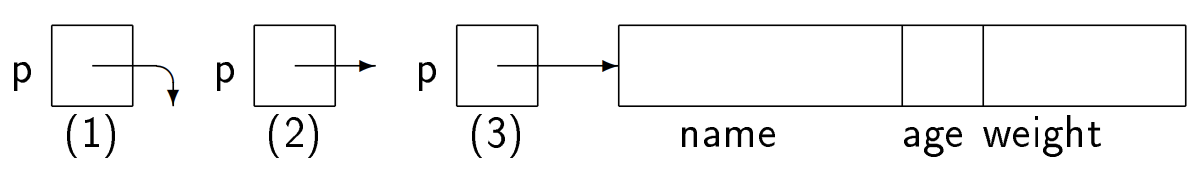
\includegraphics[scale=0.5]{./estáticos/punterosej.png}
    \caption{Casos posibles para un puntero}
    \label{fig:my_label}
\end{figure}
\begin{enumerate}
    \item El valor de $p$ es \texttt{null}, lo cual indica que no apunta a ningún bloque de memoria.
    \item La dirección de memoria a la que apunta $p$ no está reservada, por lo que no se puede acceder a ella.
    \item El valor de $p$ es una dirección de memoria reservada, por lo que se puede acceder a ella. En este caso, $\star p$ denota a la persona a la que apunta $p$ y por lo tanto se podria acceder a los campos de la persona ($\star$p.age, $\star$p.name, $\star$p.weight). Y tambien se podrian modificar los campos de la persona ($\star$p.age := 20).
\end{enumerate}
Una notación alternativa para acceder a los campos de una persona a la que apunta $p$ es $\rightarrow$, así por ejemplo en vez de $\star$p.age se puede escribir $p\rightarrow age$, tanto para leerlo como para modificarlo ($p\rightarrow age := 20$).

